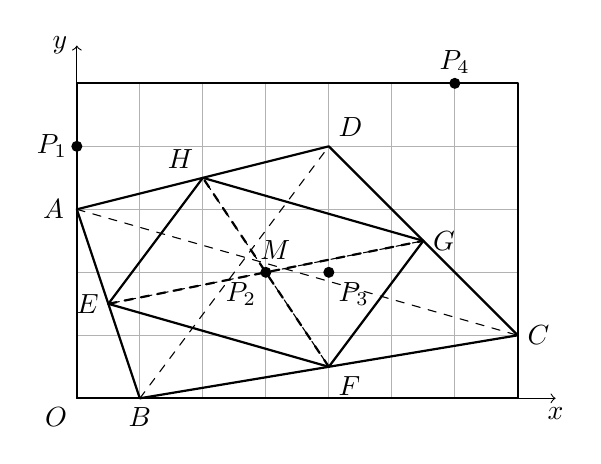
\begin{tikzpicture}[x=0.8cm,y=0.8cm,line cap=round,line join=round]
\usetikzlibrary{calc}

% grid & axes
\draw[step=1,gray!60] (0,0) grid (7,5);
\draw[thick] (0,0) rectangle (7,5);
\draw[->] (0,0) -- (7.6,0) node[below] {$x$};
\draw[->] (0,0) -- (0,5.6) node[left] {$y$};
\node[below left] at (0,0) {$O$};

% ▲ points (given)
\coordinate (A) at (0,3);
\coordinate (B) at (1,0);
\coordinate (C) at (7,1);
\coordinate (D) at (4,4);

% midpoints
\coordinate (E) at ($(A)!0.5!(B)$);
\coordinate (F) at ($(B)!0.5!(C)$);
\coordinate (G) at ($(C)!0.5!(D)$);
\coordinate (H) at ($(D)!0.5!(A)$);

% centroid / intersection
\coordinate (M) at (3,2);

% Ω points (as in the picture layout)
\coordinate (Pone)   at (0,4);   % P1
\coordinate (Ptwo)   at (3,2);   % P2 = M
\coordinate (Pthree) at (4,2);   % P3
\coordinate (Pfour)  at (6,5);   % P4

% quadrilateral ABCD
\draw[thick] (A)--(B)--(C)--(D)--cycle;

% parallelogram EFGH
\draw[thick] (E)--(F)--(G)--(H)--cycle;

% diagonals of EFGH
\draw[dashed,thick] (E)--(G);
\draw[dashed,thick] (F)--(H);

% some auxiliary dashed lines (to mimic the original style)
\draw[dashed] (A)--(C);
\draw[dashed] (B)--(D);
\draw[dashed] (M)--(E) (M)--(F) (M)--(G) (M)--(H);

% marks: ▲
\node at (A) {\Large $\blacktriangle$};
\node at (B) {\Large $\blacktriangle$};
\node at (C) {\Large $\blacktriangle$};
\node at (D) {\Large $\blacktriangle$};

% labels for A,B,C,D,E,F,G,H
\node[left] at ($(A)+(-0.05,0)$) {$A$};
\node[below] at (B) {$B$};
\node[right] at (C) {$C$};
\node[above right] at (D) {$D$};

\node[left] at (E) {$E$};
\node[below right] at (F) {$F$};
\node[right] at (G) {$G$};
\node[above left] at (H) {$H$};

% points P1..P4 (black dots)
\fill (Pone) circle (2.0pt);
\fill (Ptwo) circle (2.0pt);
\fill (Pthree) circle (2.0pt);
\fill (Pfour) circle (2.0pt);

\node[left] at ($(Pone)+(0,0)$) {$P_1$};
\node[below left] at (Ptwo) {$P_2$};
\node[below right] at (Pthree) {$P_3$};
\node[above] at (Pfour) {$P_4$};

\node[above] at ($(M)+(0.15,0.05)$) {$M$};
\node[right] at ($(0,0)+(0.05,0)$) {};
\end{tikzpicture}